%\levelB{Hardware}
The experiments did not take advantage of GPU acceleration and were  conducted on a single computer with 256GB of RAM and with 2 Intel\textregistered Xeon\textregistered E5-2630 v2 processors, with 6 cores each, with 2 hyper-threads per core, or 24 hyper-threads in total. 

%\levelB{Software}
The main software and frameworks used to build the experiments were Python 3.6 \cite{rossum_python_2019}, Jupyter notebook \cite{perez_jupyter_2019}, Tensorflow 1.14.0 \cite{google_brain_tensorflow_2019}, Keras 2.2.4-tf \cite{chollet_keras_2019}, and Fedora Linux 27.
The source code for the experiments is available at \sloppy\url{http://github.com/atilaromero/carving-experiments}.

%\levelB{Dataset}
To prepare the Govdocs1 dataset \cite{garfinkel_bringing_2009}, 200 files of each of the 28 chosen file types were randomly selected, 100 to use in the training dataset and 100 to use in the validation dataset.
%\levelB{Inputs}
A batch size of 100 was used, with 28 steps per epoch.

% \noindent
\begin{figure*}[htb!]
\centering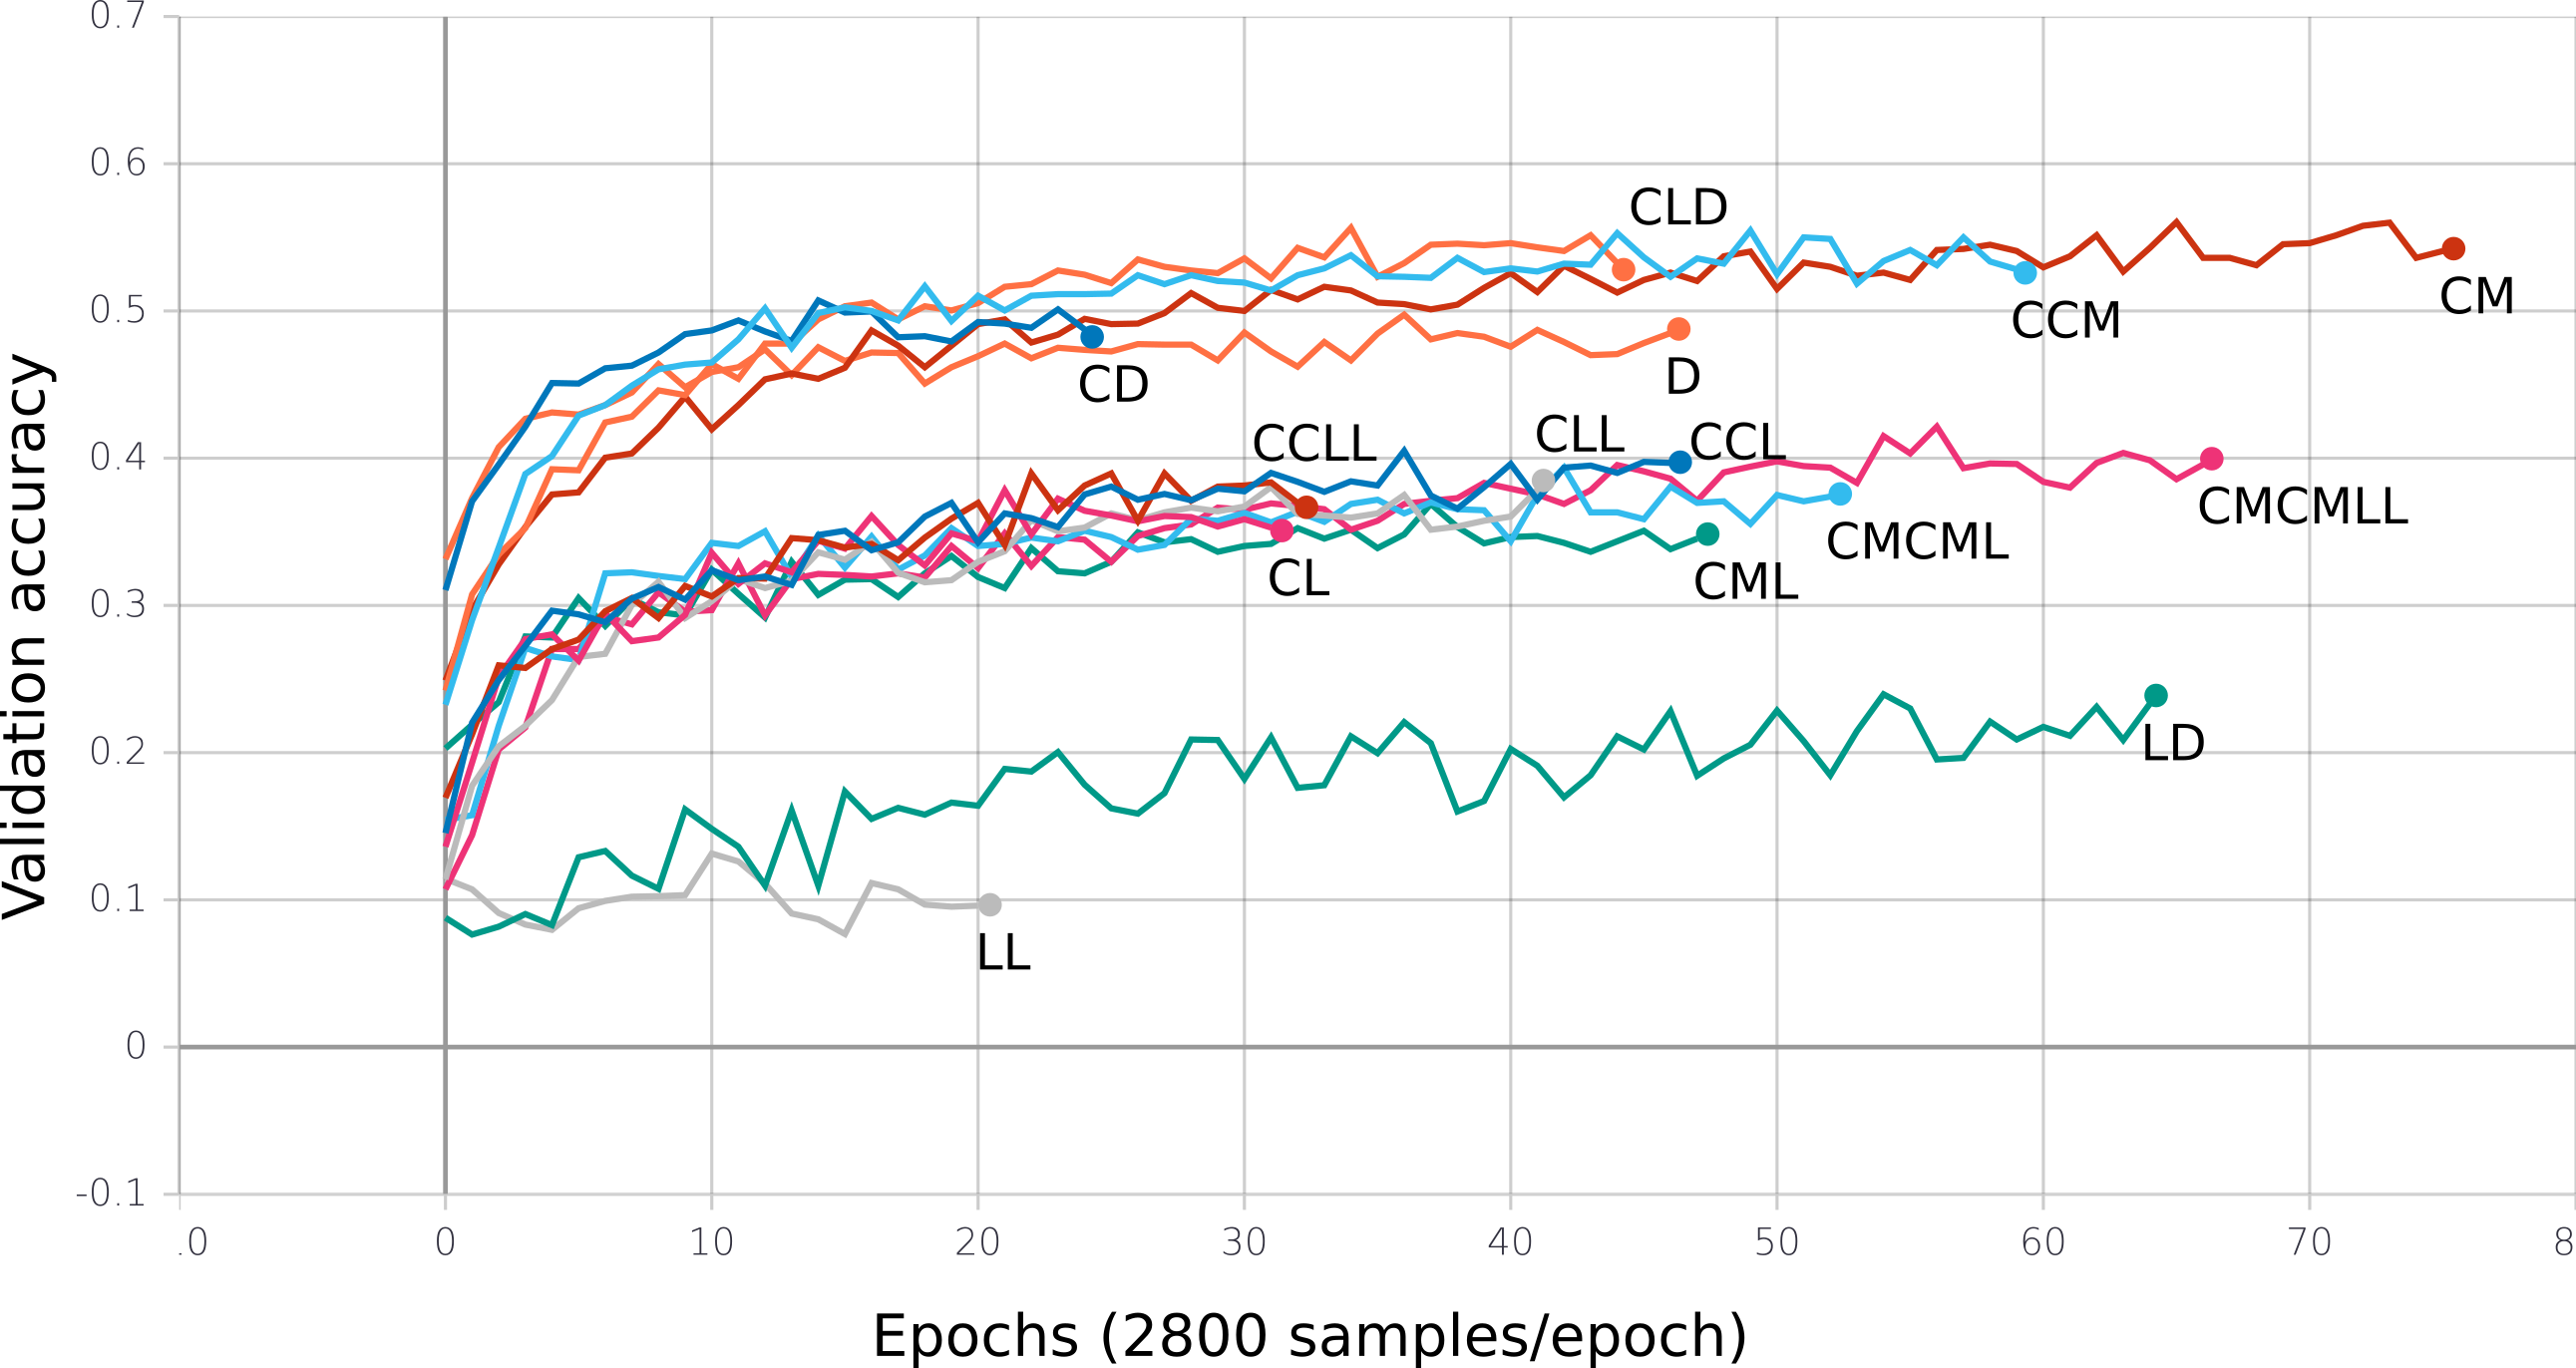
\includegraphics[width=0.9\textwidth]{content/epoch_val_categorical_accuracy.png}
\caption{\label{fig:learning}Learning curves of some models (validation accuracy vs. time)}%
\end{figure*}

%exp18
The two models that used LSTM layers without convolutional layers presented slower learning in comparison with the others, as can be seen in Figure \ref{fig:learning}.  
The final validation accuracy values can be consulted in Figure \ref{fig:models}, in which
the bar plot shows the validation accuracy of the considered models. Their training time, in minutes, and the total epochs processed is also indicated. The training was interrupted when no further improvement was observed for 10 consecutive epochs.

% \noindent
\begin{figure*}[htb!]
\centering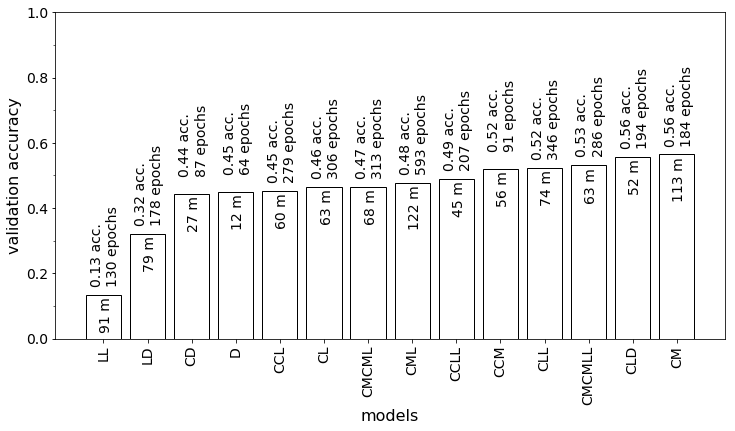
\includegraphics[width=1.0\textwidth]{content/models.png}
\caption[Validation accuracy of models]{\label{fig:models}The bar plot shows the validation accuracy of the considered models. Their training time, in minutes, and the total epochs processed is also indicated. The training was interrupted when no further improvement was observed for 10 consecutive epochs.}%
\end{figure*}

The validation accuracy values of the remaining models were in the 35\%-54\% range.
{\color{red}
To check if the two slower models could give better results if executed for a longer period, they were trained for 10 hours. The model identified as ``LD'', which uses an LSTM layer followed by a fully connected layer, was able to achieve an accuracy of 49.4\%, while the other, ``LL'', achieved only 15.3\%.
}

% \levelC{Limitations and threats to validity}
The model ``CLD'' was chosen to be compared with other works because it was among the three models with the highest accuracy, but achieved its results in less time and showed high resilience to changes in parameters during the tests, while the others did not.

In a second stage, a longer training session was performed, using a batch size of 300 samples instead of 100, and increasing the improvement threshold of the early stopping condition (maximum number of epochs to wait for improvements) from 10 to 20. These parameters were chosen by trial and error. For the initial 28 file types, the ``CLD'' model training time increased from eight minutes to three hours using these parameters.

Using longer training sessions, the accuracy for the 28 file types used in the first stage increased from 54\% to 63\%. Using the same file types of other works, the ``CLD'' model achieved an accuracy of 
67\% for the file types from Chen \textit{et al.} \cite{chen_file_2018},
91\% for Hiester \cite{hiester_file_2018}, 
59\% for Wang \textit{et al.} \cite{wang_sparse_2018},
65\% for Wang \textit{et al.} \cite{wang_file_2018},
and
61\% for Vulinović \textit{et al.} \cite{vulinovic_neural_2019}.
The results can be seen in Figure \ref{fig:cldothers}, in which the bar plot shows the comparison between the validation accuracy obtained with ``CLD'' and those achieved in other studies.

\noindent
\begin{figure*}[htb!]
\centering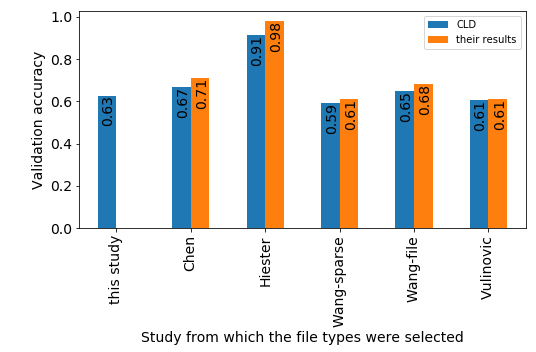
\includegraphics[width=0.8\textwidth]{content/CLD-others.png}
\caption[CLD vs. other studies]{\label{fig:cldothers}The ``CLD'' model was trained from scratch using the same file types used in other works. The bar plot shows the comparison between the validation accuracy obtained with ``CLD'' and those achieved in other studies.}%
\end{figure*}
